\documentclass[11pt,a4paper]{article}

\usepackage[T1]{fontenc}
\usepackage[utf8]{inputenc}
\usepackage[sc]{mathpazo}
\linespread{1.06}
\usepackage{amsmath,amssymb,mathtools}
\usepackage[a4paper,margin=2.6cm,headheight=14pt]{geometry}
\usepackage{tikz}
\usetikzlibrary{arrows.meta,positioning,decorations.pathmorphing,calc}
\usepackage[most]{tcolorbox}
\usepackage{enumitem}
\usepackage{booktabs}
\usepackage{microtype}
\usepackage{fancyhdr}
\usepackage[colorlinks=true,linkcolor=azulesc,citecolor=azulesc,urlcolor=azulesc]{hyperref}

% ---------- cores ----------
\definecolor{azulesc}{HTML}{1F3864}
\definecolor{azulclaro}{HTML}{E8EEF7}
\definecolor{vermelhoesc}{HTML}{8B2500}
\definecolor{vermelhoclaro}{HTML}{FBEAE3}
\definecolor{verdeesc}{HTML}{1F5C3A}
\definecolor{verdeclaro}{HTML}{E6F2EA}
\definecolor{cinza}{HTML}{5A5A5A}
\definecolor{ocre}{HTML}{B8860B}

% ---------- cabecalho ----------
\pagestyle{fancy}
\fancyhf{}
\fancyhead[L]{\small\color{cinza}Do zero ao trímero — Parte I}
\fancyhead[R]{\small\color{cinza}\thepage}
\renewcommand{\headrulewidth}{0.4pt}

% ---------- caixas ----------
\newtcolorbox{suavez}[1][]{
  enhanced, breakable,
  colback=vermelhoclaro, colframe=vermelhoesc,
  boxrule=0.9pt, arc=2pt, left=10pt,right=10pt,top=8pt,bottom=8pt,
  fonttitle=\bfseries\sffamily,
  title={Sua vez\ #1}}

\newtcolorbox{atencao}[1][]{
  enhanced, breakable,
  colback=white, colframe=ocre,
  boxrule=0.9pt, arc=2pt, left=10pt,right=10pt,top=8pt,bottom=8pt,
  fonttitle=\bfseries\sffamily,
  title={#1}}

\newtcolorbox{ideia}[1][]{
  enhanced, breakable,
  colback=azulclaro, colframe=azulesc,
  boxrule=0.9pt, arc=2pt, left=10pt,right=10pt,top=8pt,bottom=8pt,
  fonttitle=\bfseries\sffamily,
  title={#1}}

\newtcolorbox{ponte}[1][]{
  enhanced, breakable,
  colback=verdeclaro, colframe=verdeesc,
  boxrule=0.9pt, arc=2pt, left=10pt,right=10pt,top=8pt,bottom=8pt,
  fonttitle=\bfseries\sffamily,
  title={#1}}

% ---------- atalhos ----------
\newcommand{\hbtm}{\frac{\hbar^{2}}{2m_{r}}}
\newcommand{\dd}{\mathrm{d}}
\renewcommand{\vec}[1]{\mathbf{#1}}

\setlength{\parskip}{0.35em}

\title{\vspace{-1.5cm}\Huge\bfseries Do zero ao trímero\\[0.25cm]
\LARGE\mdseries Parte I — uma partícula, duas partículas}
\author{\large Notas de estudo · Pedro Henrique G. Modesto\\[0.15cm]
\normalsize Mestrado IFSC/USP · orientação: Lucas Madeira}
\date{\normalsize Agosto de 2026}

\begin{document}
\maketitle
\thispagestyle{empty}

\begin{ideia}[Como usar este texto]
As deduções aqui estão \textbf{fechadas} — você pode ler de ponta a ponta sem travar.
Em quatro pontos há uma caixa vermelha \textbf{Sua vez}: são passos curtos (duas a
quatro linhas cada), escolhidos porque o \emph{prazer} de fechá-los é maior que a
dificuldade. Faça-os com caneta, no papel, sem consultar o resto.

Os quatro juntos dão menos de meia hora. Se algum travar por mais de dez minutos,
é sinal de que faltou algo \emph{antes} — volte, não force.
\end{ideia}

\vspace{0.3cm}

\section*{Onde estamos indo}
\addcontentsline{toc}{section}{Onde estamos indo}

O trímero de Efimov não é um assunto difícil por causa da conta. Ele é difícil
porque exige que cinco coisas estejam firmes ao mesmo tempo. Este texto trata das
três primeiras, que são as de \emph{um} e \emph{dois} corpos.

\begin{center}
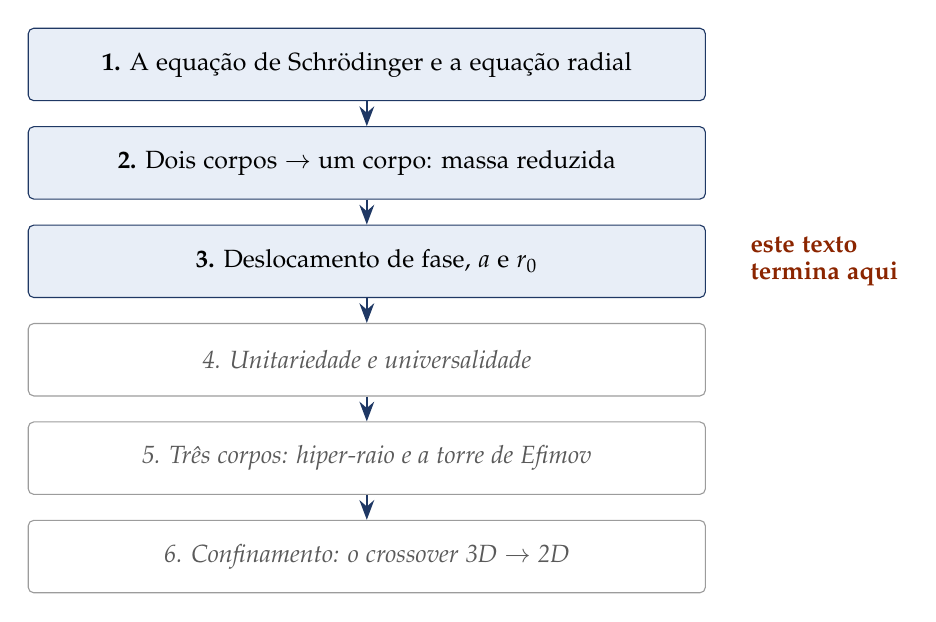
\begin{tikzpicture}[
  degrau/.style={draw=azulesc, fill=azulclaro, rounded corners=2pt,
                 minimum width=8.6cm, minimum height=0.92cm, align=center,
                 font=\small},
  futuro/.style={draw=cinza!60, fill=white, rounded corners=2pt,
                 minimum width=8.6cm, minimum height=0.92cm, align=center,
                 font=\small\itshape, text=cinza},
  seta/.style={-{Stealth[length=2.5mm]}, azulesc, thick}
]
\node[degrau] (d1) at (0,0) {\textbf{1.} A equação de Schrödinger e a equação radial};
\node[degrau] (d2) at (0,-1.25) {\textbf{2.} Dois corpos $\to$ um corpo: massa reduzida};
\node[degrau] (d3) at (0,-2.5) {\textbf{3.} Deslocamento de fase, $a$ e $r_{0}$};
\node[futuro] (d4) at (0,-3.75) {4. Unitariedade e universalidade};
\node[futuro] (d5) at (0,-5.0) {5. Três corpos: hiper-raio e a torre de Efimov};
\node[futuro] (d6) at (0,-6.25) {6. Confinamento: o crossover 3D $\to$ 2D};
\draw[seta] (d1) -- (d2);
\draw[seta] (d2) -- (d3);
\draw[seta] (d3) -- (d4);
\draw[seta] (d4) -- (d5);
\draw[seta] (d5) -- (d6);
\node[right=0.35cm of d3, font=\small\bfseries, text=vermelhoesc, align=left]
  {\ este texto\\[-1pt] \ termina aqui};
\end{tikzpicture}
\end{center}

\begin{ponte}[O que o Lucas espera que esteja firme antes do trímero]
Não é ``saber Efimov''. É saber responder, sem consultar:
\begin{enumerate}[leftmargin=*, itemsep=1pt, topsep=2pt]
\item Por que dois corpos viram um, e qual massa entra na conta.
\item Por que um potencial central só consegue \emph{deslocar a fase} da onda.
\item O que é o comprimento de espalhamento \emph{geometricamente}.
\item Por que $a$ pode ser infinito com um potencial perfeitamente finito.
\item O que $r_{0}$ mede, e por que ele é a correção seguinte.
\item Por que a baixa energia colapsa o problema em um único número.
\end{enumerate}
Todas as seis são respondidas aqui.
\end{ponte}

\newpage
\tableofcontents
\newpage

% =====================================================================
\section{Uma partícula}
% =====================================================================

\subsection{A equação, e o que se pergunta a ela}

Uma partícula de massa $m$ num potencial $V(\vec r)$ obedece
\begin{equation}
\left[-\frac{\hbar^{2}}{2m}\nabla^{2} + V(\vec r)\right]\psi(\vec r) = E\,\psi(\vec r).
\label{eq:schr}
\end{equation}

Antes de qualquer conta, o ponto conceitual que organiza tudo: \eqref{eq:schr} é a
mesma equação para estados ligados e para espalhamento, mas \textbf{a pergunta é
diferente nos dois casos}.

\begin{center}
\begin{tabular}{@{}p{0.44\textwidth}p{0.44\textwidth}@{}}
\toprule
\textbf{Estado ligado} ($E<0$) & \textbf{Espalhamento} ($E>0$) \\
\midrule
$\psi$ é normalizável, decai como $e^{-\kappa r}$. & $\psi$ não é normalizável; oscila até o infinito.\\[3pt]
Só existe solução para \emph{alguns} $E$. O espectro é discreto. & Existe solução para \emph{todo} $E>0$. O espectro é contínuo.\\[3pt]
A pergunta é: \emph{quais são as energias?} & A pergunta é: \emph{fixada a energia, qual é a solução com a condição de contorno certa?}\\
\bottomrule
\end{tabular}
\end{center}

Guarde isso: em espalhamento, procurar autovalores não faz sentido — eles são todos.
O que se procura é a \emph{forma} da solução longe do alvo.

\subsection{Potencial central: a equação radial}

Se $V=V(r)$ depende só da distância, o momento angular se conserva. Em coordenadas
esféricas o laplaciano se separa,
\begin{equation}
\nabla^{2} = \frac{1}{r^{2}}\frac{\partial}{\partial r}\!\left(r^{2}\frac{\partial}{\partial r}\right)
- \frac{\vec L^{2}}{\hbar^{2}r^{2}},
\end{equation}
e como $[\hat H,\vec L^{2}]=[\hat H,\hat L_{z}]=0$, podemos procurar soluções que sejam
autofunções simultâneas dos três operadores:
\begin{equation}
\psi(\vec r) = R_{l}(r)\,Y_{lm}(\theta,\varphi),
\qquad \vec L^{2}Y_{lm} = \hbar^{2}l(l+1)Y_{lm}.
\end{equation}
Substituindo em \eqref{eq:schr}:
\begin{equation}
R_{l}'' + \frac{2}{r}R_{l}' + \left[k^{2} - U(r) - \frac{l(l+1)}{r^{2}}\right]R_{l}=0,
\qquad
k^{2}\equiv\frac{2mE}{\hbar^{2}},\quad U\equiv\frac{2mV}{\hbar^{2}}.
\end{equation}

\subsection{O truque \texorpdfstring{$u=rR$}{u = rR}}

O termo $\tfrac{2}{r}R'$ é um estorvo: ele estraga a analogia com uma equação
unidimensional e atrapalha a integração numérica. A substituição
\begin{equation}
\boxed{\;u_{l}(r) = r\,R_{l}(r)\;}
\end{equation}
o elimina exatamente. De fato, $u'' = rR'' + 2R'$, e portanto
\begin{equation}
\boxed{\;u_{l}''(r) + \left[k^{2} - U(r) - \frac{l(l+1)}{r^{2}}\right]u_{l}(r) = 0\;}
\label{eq:radial}
\end{equation}

\begin{ideia}[Por que esta é \emph{a} equação do seu laboratório]
A Eq.~\eqref{eq:radial} tem a forma $u'' = f(r)\,u$, sem primeira derivada. Essa é
precisamente a classe de equações para a qual o método de Numerov foi construído, e
é por isso que ele aparece em todo o seu código. O preço da substituição é a
condição $u_{l}(0)=0$, que é apenas o requisito de que $R_{l}$ seja finito na origem.
\end{ideia}

\subsection{Comportamento na origem e a barreira centrífuga}

Perto de $r=0$, se $U$ for menos singular que $1/r^{2}$, o termo dominante em
\eqref{eq:radial} é o centrífugo:
\begin{equation}
u_{l}'' \simeq \frac{l(l+1)}{r^{2}}u_{l}
\quad\Longrightarrow\quad
u_{l}\sim r^{\,l+1} \ \ \text{ou}\ \ u_{l}\sim r^{-l}.
\end{equation}
A segunda solução é descartada: para $l\ge1$ ela diverge, e mesmo para $l=0$ ela dá
$R_{0}\sim 1/r$, que não satisfaz a equação de Schrödinger na origem. Fica
\begin{equation}
u_{l}(r) \xrightarrow[\;r\to0\;]{} r^{\,l+1}.
\label{eq:origem}
\end{equation}
Quanto maior $l$, mais a função de onda é \emph{empurrada para fora} da região onde o
potencial existe. Essa é a raiz física de tudo que faremos em baixa energia.

\subsection{O exemplo âncora: o poço esférico}

Tome $V(r) = -V_{0}$ para $r<R$ e $0$ fora, com $l=0$. Em energia zero, dentro do poço
$u'' = -K_{0}^{2}u$ com $K_{0}=\sqrt{2mV_{0}}/\hbar$, e fora $u''=0$. Logo
\begin{equation}
u(r) = \begin{cases}
A\sin(K_{0}r), & r<R \quad\text{(já satisfaz } u(0)=0),\\[4pt]
B\,(r-a), & r>R \quad\text{(a solução geral de } u''=0).
\end{cases}
\end{equation}
Emendar as duas em $r=R$ significa casar a \emph{derivada logarítmica} $u'/u$ — que é
o que não depende da normalização:
\begin{equation}
K_{0}\cot(K_{0}R) = \frac{1}{R-a}.
\label{eq:casamento}
\end{equation}

\begin{suavez}[\;1 — o comprimento de espalhamento do poço]
Isole $a$ na Eq.~\eqref{eq:casamento}. Você deve chegar em
\[
a = R - \frac{\tan(K_{0}R)}{K_{0}}.
\]
Agora responda \emph{sem calcular}: o que acontece com $a$ quando $K_{0}R\to\pi/2$?
E o que você acha que está fisicamente ocorrendo com o poço nesse momento?

\vspace{2.2cm}
\hrulefill
\end{suavez}

Aquilo que você acabou de encontrar é o fenômeno central do resto do texto: em
$K_{0}R=\pi/2$ o poço fica \emph{exatamente} fundo o bastante para segurar o primeiro
estado ligado, e $a$ diverge. Voltaremos a isso na Seção~\ref{sec:divergencia} com
todo o cuidado que ele merece.

% =====================================================================
\section{Duas partículas}
% =====================================================================

\subsection{A redução exata}

Dois átomos interagindo por um potencial que depende só da separação:
\begin{equation}
\hat H = \frac{\vec p_{1}^{\,2}}{2m_{1}} + \frac{\vec p_{2}^{\,2}}{2m_{2}} + V(|\vec r_{1}-\vec r_{2}|).
\end{equation}
Definindo centro de massa e coordenada relativa,
\begin{equation}
\vec R = \frac{m_{1}\vec r_{1}+m_{2}\vec r_{2}}{M},\qquad
\vec r = \vec r_{1}-\vec r_{2},\qquad
M=m_{1}+m_{2},\qquad
m_{r}=\frac{m_{1}m_{2}}{m_{1}+m_{2}},
\end{equation}
a álgebra dá, \emph{exatamente} e sem aproximação nenhuma,
\begin{equation}
\hat H = \underbrace{\frac{\vec P^{2}}{2M}}_{\text{livre}} \;+\; \underbrace{\frac{\vec p^{\,2}}{2m_{r}} + V(r)}_{\text{o problema de verdade}}.
\end{equation}
O centro de massa é uma partícula livre e não sabe que houve colisão. Todo o
espalhamento vive na parte relativa, que é o problema de \emph{uma} partícula da
Seção 1 com $m\to m_{r}$:
\begin{equation}
\left[-\hbtm\nabla^{2}+V(r)\right]\psi(\vec r)=E\,\psi(\vec r),
\qquad E=\frac{\hbar^{2}k^{2}}{2m_{r}}.
\end{equation}

\begin{atencao}[Onde este assunto mais sangra: o fator 2]
Para dois átomos \emph{idênticos} (o seu caso, $^{39}$K), $m_{1}=m_{2}=m$ e portanto
\[
m_{r}=\frac{m}{2}
\qquad\Longrightarrow\qquad
\hbtm=\frac{\hbar^{2}}{m}.
\]
Os dois lados dessa igualdade aparecem impressos na literatura, e nem sempre com a
mesma convenção de $U$. Você já foi mordido por isso \textbf{duas vezes}: o fator 2
das constantes do Lennard-Jones e o $2m_{r}$ que faltava na definição de
$\ell_{\mathrm{vdW}}$.

\textbf{Regra:} quando um número não bater por $2$, $\sqrt{2}$ ou $4$, o suspeito
número um é a convenção de massa. Verifique-a \emph{antes} de procurar bug.
\end{atencao}

\subsection{A condição de contorno: onde o espalhamento começa}

O enunciado físico do experimento é: longe do alvo há uma onda plana chegando e uma
onda esférica saindo.
\begin{equation}
\psi(\vec r) \xrightarrow[\;r\to\infty\;]{}
e^{ikz} + f(\theta)\,\frac{e^{ikr}}{r}.
\label{eq:assint}
\end{equation}

\begin{center}
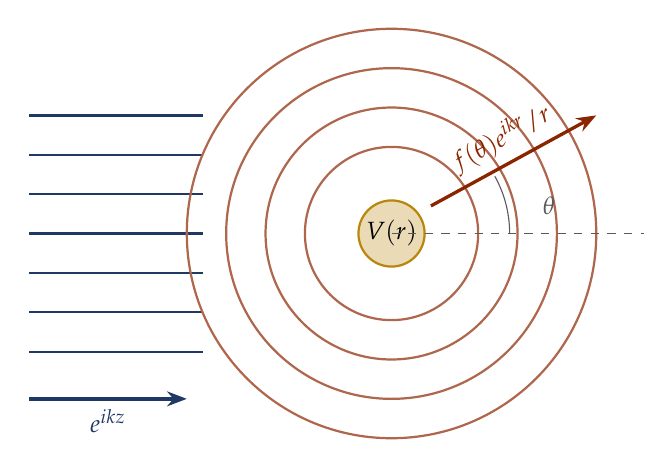
\begin{tikzpicture}[scale=1.0]
\foreach \y in {-1.5,-1.0,...,1.5}{
  \draw[azulesc, thick] (-4.6,\y) -- (-2.4,\y);
}
\foreach \rr in {1.1,1.6,2.1,2.6}{
  \draw[vermelhoesc!70, thick] (0,0) circle (\rr);
}
\filldraw[fill=ocre!30, draw=ocre, thick] (0,0) circle (0.42);
\node at (0,0) {\small $V(r)$};
\draw[-{Stealth[length=2.5mm]}, very thick, azulesc] (-4.6,-2.1) -- (-2.6,-2.1)
      node[midway, below, font=\small] {$e^{ikz}$};
\draw[-{Stealth[length=2.5mm]}, very thick, vermelhoesc] (0.5,0.35) -- (2.6,1.5)
      node[midway, above, sloped, font=\small] {$f(\theta)e^{ikr}/r$};
\draw[dashed, cinza] (0,0) -- (3.2,0);
\draw[cinza] (1.5,0) arc (0:29:1.5);
\node[cinza, font=\small] at (2.0,0.35) {$\theta$};
\end{tikzpicture}
\end{center}

Três observações, todas verificáveis:

\begin{itemize}[leftmargin=*, itemsep=2pt]
\item \textbf{Por que $1/r$?} Conservação de fluxo. A onda esférica atravessa uma casca
de área $4\pi r^{2}$; para a corrente total não depender de $r$, precisamos
$|\psi|^{2}\propto 1/r^{2}$, logo $\psi\propto 1/r$. Não é escolha estética, é
contabilidade.
\item \textbf{Por que só $\theta$?} Porque $V$ é central \emph{e} a onda incidente
elegeu o eixo $z$. A simetria remanescente é rotação em torno de $z$.
\item \textbf{Quando isso falha:} \eqref{eq:assint} exige $V$ decaindo mais rápido que
$1/r$. Coulomb quebra (aparece um logaritmo na fase). Para você, $-C_{6}/r^{6}$ está
folgadamente dentro — e note que o critério de ``curto alcance'' de Efimov é mais
exigente, mais rápido que $1/r^{3}$, porque três corpos pedem mais.
\end{itemize}

Comparando a corrente espalhada com a incidente obtém-se, sem esforço,
\begin{equation}
\frac{\dd\sigma}{\dd\Omega} = |f(\theta)|^{2}.
\end{equation}
Portanto \textbf{todo o problema é calcular $f$}.

\subsection{Ondas parciais e a ideia central de todo o assunto}

Como $V$ é central, cada momento angular é um canal independente: o potencial não
mistura $l$'s. Podemos então resolver um $l$ de cada vez, usando exatamente a
Eq.~\eqref{eq:radial}.

Fora do alcance do potencial, $U=0$, e a equação radial é livre. A solução livre
regular é $u_{l}\propto kr\,j_{l}(kr)$, cuja forma assintótica é
\begin{equation}
u_{l}^{\text{livre}}(r)\xrightarrow[\;r\to\infty\;]{} \sin\!\left(kr-\frac{l\pi}{2}\right).
\end{equation}
Com potencial, \emph{longe dele} a equação é a mesma. Então a solução só pode diferir
por amplitude e fase:
\begin{equation}
\boxed{\;u_{l}(r)\xrightarrow[\;r\to\infty\;]{} C_{l}\,\sin\!\left(kr-\frac{l\pi}{2}+\delta_{l}\right)\;}
\label{eq:fase}
\end{equation}

\begin{ideia}[O resultado mais importante da teoria de espalhamento elástico]
Um potencial central \textbf{não pode fazer nada com a onda além de empurrar a fase
dela}.

Não pode mudar a amplitude relativa dos canais: isso violaria conservação de fluxo
(elástico significa que tudo que entra sai). Não pode misturar $l$'s: a simetria
proíbe. Logo, \emph{tudo} que um potencial central faz num experimento de
espalhamento elástico cabe numa lista de números $\delta_{0},\delta_{1},\delta_{2},\dots$

Consequência que vale parar para digerir: \textbf{dois potenciais completamente
diferentes com os mesmos $\delta_{l}$ são experimentalmente indistinguíveis.}

É exatamente daqui — e de nenhum outro lugar — que nasce a palavra
\emph{universalidade} que domina a sua dissertação. Quando você troca o Lennard-Jones
por um gaussiano e obtém a mesma física de baixa energia, não é coincidência nem
sorte numérica: é este teorema.
\end{ideia}

Falta ligar $\delta_{l}$ a $f(\theta)$. Usa-se a expansão de Rayleigh da onda plana,
\begin{equation}
e^{ikz} = \sum_{l=0}^{\infty} i^{l}(2l+1)\,j_{l}(kr)\,P_{l}(\cos\theta),
\end{equation}
escreve-se $\psi$ também em ondas parciais, e comparam-se os coeficientes das
exponenciais $e^{\pm ikr}$ termo a termo. O resultado:
\begin{equation}
\boxed{\;f(\theta) = \frac{1}{k}\sum_{l=0}^{\infty}(2l+1)\,e^{i\delta_{l}}\sin\delta_{l}\,P_{l}(\cos\theta)\;}
\end{equation}
e, integrando $|f|^{2}$ com a ortogonalidade dos $P_{l}$,
\begin{equation}
\sigma = \frac{4\pi}{k^{2}}\sum_{l}(2l+1)\sin^{2}\delta_{l},
\qquad\text{e como caso particular}\qquad
\sigma = \frac{4\pi}{k}\,\mathrm{Im}\,f(0),
\end{equation}
esta última sendo o \emph{teorema óptico}.

\subsection{Baixa energia: por que sobra um número só}

Classicamente, uma partícula com momento $\hbar k$ e momento angular $\hbar l$ passa a
uma distância $b\approx l/k$ do alvo. Se $b$ for muito maior que o alcance $R_{V}$ do
potencial, ela não o viu. Logo só contribuem
\begin{equation}
l \lesssim k R_{V}.
\end{equation}
Quanticamente, o mesmo sai de \eqref{eq:origem}: a barreira centrífuga sufoca
$u_{l}\sim r^{l+1}$ na região onde $V$ vive. A versão quantitativa é a
\textbf{lei de limiar de Wigner},
\begin{equation}
\tan\delta_{l} \propto k^{2l+1}\qquad (k\to0),
\end{equation}
que você vai deduzir na sessão de ondas parciais.

\begin{center}
\emph{Quando $kR_{V}\ll1$, apenas $l=0$ espalha.}
\end{center}

Para átomos ultrafrios isso não é uma aproximação acadêmica: é o regime de trabalho.
E é por isso que a onda-$s$ é o assunto inteiro.

\subsection{O comprimento de espalhamento}

Se só $l=0$ importa e $\delta_{0}\to0$ quando $k\to0$, o conteúdo todo está no
primeiro coeficiente do desenvolvimento. Define-se
\begin{equation}
\boxed{\;\delta_{0}(k) \xrightarrow[\;k\to0\;]{} -\,k\,a\;}
\label{eq:defa}
\end{equation}
Com isso $f\to -a$, isotrópico — a baixa energia o alvo não tem forma, só tamanho — e
\begin{equation}
\sigma \xrightarrow[\;k\to0\;]{} 4\pi a^{2}.
\end{equation}

\begin{suavez}[\;2 — a leitura geométrica de $a$]
Parta de $u_{0}(r)\propto\sin(kr+\delta_{0})$, válida fora do alcance do potencial.
Substitua \eqref{eq:defa}, tome $k\to0$ e mostre que
\[
u_{0}(r)\ \propto\ r-a
\qquad\text{(fora do alcance).}
\]
São três linhas: use $\sin x\approx x$ para argumento pequeno.

\vspace{2.0cm}
\hrulefill
\end{suavez}

O que você acabou de provar é a maneira certa de pensar em $a$ pelo resto do
mestrado. Em energia zero, fora do potencial, a equação é $u''=0$ — uma reta. E:

\begin{center}
\fbox{\parbox{0.85\textwidth}{\centering
$a$ é \textbf{onde a reta assintótica cruza o eixo}, extrapolada para dentro.\\
Só isso. Uma esfera dura de raio $a$ dá exatamente $a$, porque a função é obrigada a
zerar ali.}}
\end{center}

\begin{figure}[htbp]
\centering
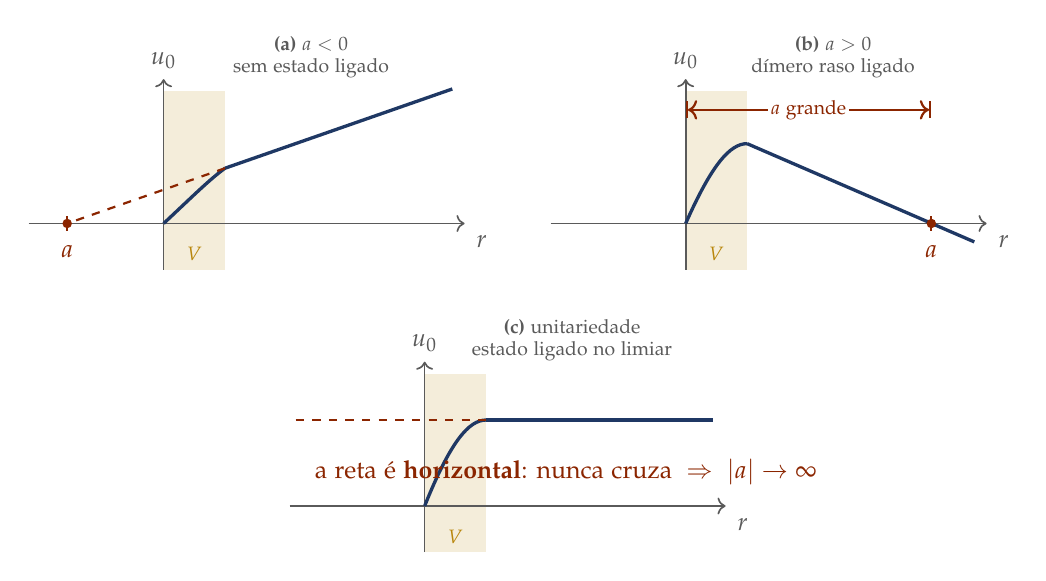
\begin{tikzpicture}[scale=0.78,
  eixo/.style={->, cinza, semithick},
  onda/.style={azulesc, very thick},
  extrap/.style={vermelhoesc, thick, dashed},
  rot/.style={font=\scriptsize, text=cinza}]

% ================= painel A : a < 0 =================
\begin{scope}[xshift=0cm]
  \fill[ocre!15] (0,-0.75) rectangle (1.0,2.15);
  \draw[eixo] (-2.2,0) -- (4.9,0) node[below right=1pt, font=\small] {$r$};
  \draw[eixo] (0,-0.75) -- (0,2.35) node[above, font=\small] {$u_0$};
  \node[ocre, font=\scriptsize] at (0.5,-0.5) {$V$};
  % funcao dentro + fora
  \draw[onda] (0,0) .. controls (0.45,0.42) and (0.75,0.72) .. (1.0,0.90);
  \draw[onda] (1.0,0.90) -- (4.7,2.19);
  % extrapolacao para tras
  \draw[extrap] (1.0,0.90) -- (-1.57,0);
  \fill[vermelhoesc] (-1.57,0) circle (2.2pt);
  \draw[vermelhoesc, thick] (-1.57,-0.12) -- (-1.57,0.12);
  \node[vermelhoesc, font=\small] at (-1.57,-0.45) {$a$};
  \node[rot, align=center] at (2.4,2.7) {\textbf{(a)} $a<0$\\ sem estado ligado};
\end{scope}

% ================= painel B : a > 0 grande =================
\begin{scope}[xshift=8.5cm]
  \fill[ocre!15] (0,-0.75) rectangle (1.0,2.15);
  \draw[eixo] (-2.2,0) -- (4.9,0) node[below right=1pt, font=\small] {$r$};
  \draw[eixo] (0,-0.75) -- (0,2.35) node[above, font=\small] {$u_0$};
  \node[ocre, font=\scriptsize] at (0.5,-0.5) {$V$};
  \draw[onda] (0,0) .. controls (0.42,0.95) and (0.72,1.30) .. (1.0,1.30);
  \draw[onda] (1.0,1.30) -- (4.7,-0.30);
  \fill[vermelhoesc] (4.0,0) circle (2.2pt);
  \draw[vermelhoesc, thick] (4.0,-0.12) -- (4.0,0.12);
  \node[vermelhoesc, font=\small] at (4.0,-0.45) {$a$};
  \draw[vermelhoesc, thick, |<->|] (0,1.85) -- (4.0,1.85);
  \node[vermelhoesc, font=\scriptsize, fill=white, inner sep=1pt] at (2.0,1.85) {$a$ grande};
  \node[rot, align=center] at (2.4,2.7) {\textbf{(b)} $a>0$\\ dímero raso ligado};
\end{scope}

% ================= painel C : unitariedade =================
\begin{scope}[xshift=4.25cm, yshift=-4.6cm]
  \fill[ocre!15] (0,-0.75) rectangle (1.0,2.15);
  \draw[eixo] (-2.2,0) -- (4.9,0) node[below right=1pt, font=\small] {$r$};
  \draw[eixo] (0,-0.75) -- (0,2.35) node[above, font=\small] {$u_0$};
  \node[ocre, font=\scriptsize] at (0.5,-0.5) {$V$};
  \draw[onda] (0,0) .. controls (0.42,1.05) and (0.72,1.40) .. (1.0,1.40);
  \draw[onda] (1.0,1.40) -- (4.7,1.40);
  \draw[extrap] (-2.1,1.40) -- (1.0,1.40);
  \node[vermelhoesc, font=\small, align=center] at (2.3,0.55)
    {a reta é \textbf{horizontal}: nunca cruza $\;\Rightarrow\; |a|\to\infty$};
  \node[rot, align=center] at (2.4,2.7) {\textbf{(c)} unitariedade\\ estado ligado no limiar};
\end{scope}

\end{tikzpicture}

\vspace{0.3cm}
\begin{minipage}{0.88\textwidth}
\small\color{cinza}
\textbf{Figura 2.} A função de onda de energia zero. Dentro do alcance do potencial
(faixa clara) ela curva; fora, a equação é $u''=0$ e ela é uma \emph{reta}. O
comprimento de espalhamento é o ponto onde essa reta cruza o eixo. Aumentar a
profundidade do poço faz a reta girar: o cruzamento passeia para a direita, vai a
$+\infty$, e reaparece em $-\infty$ — tudo com o potencial variando suavemente.
\end{minipage}
\end{figure}

\subsection{Por que \texorpdfstring{$a$}{a} pode ser infinito}
\label{sec:divergencia}

Aqui está o fato que governa Feshbach, Efimov e o seu projeto inteiro.

Torne o poço um pouco mais fundo. A função de onda interna curva um pouco mais, sai
com derivada logarítmica um pouco menor, e a reta externa \emph{gira}. O ponto onde
ela cruza o eixo passeia — e pode ir a $+\infty$, reaparecer em $-\infty$, tudo isso
com o potencial variando suavemente e permanecendo perfeitamente finito.

Quando o poço fica fundo o bastante para \emph{quase} segurar um estado ligado, a reta
sai horizontal e $|a|\to\infty$. Foi exatamente o que você achou na
\textbf{Sua vez 1}, em $K_{0}R=\pi/2$.

\begin{center}
\fbox{\parbox{0.88\textwidth}{\centering\bfseries
Comprimento de espalhamento divergente $\;\Longleftrightarrow\;$ estado ligado
exatamente no limiar.}}
\end{center}

Este é o ponto de contato com o seu laboratório e com o experimento da Patrícia: é o
que a ressonância de Feshbach faz com um ímã, e é a condição sob a qual Efimov
encontrou a torre infinita.

Podemos ser quantitativos. A amplitude de onda-$s$ é
$f = \left(k\cot\delta_{0}-ik\right)^{-1}$, e um estado ligado é um \emph{polo} de $f$
em $k=i\kappa$ com $\kappa>0$, correspondendo a $u\sim e^{-\kappa r}$ e energia
$E_{b}=-\hbar^{2}\kappa^{2}/2m_{r}$. Usando $k\cot\delta_{0}\simeq-1/a$:
\begin{equation}
-\frac{1}{a} + \kappa = 0
\qquad\Longrightarrow\qquad
\kappa \simeq \frac{1}{a}.
\end{equation}

\begin{suavez}[\;3 — a energia do dímero raso]
Da relação $\kappa\simeq 1/a$ que acabamos de obter, escreva $E_{b}$ em função de $a$.
\[
E_{b} \;=\; -\,\frac{\hbar^{2}\kappa^{2}}{2m_{r}} \;=\; \rule{3.5cm}{0.4pt}
\]
Depois responda: se $a>0$ e muito grande, o dímero é fortemente ou fracamente ligado?
E o tamanho típico dele é da ordem de quê?

\vspace{1.8cm}
\hrulefill
\end{suavez}

O que você obteve é a fórmula que conecta o seu módulo \texttt{feshbach.py} ao
experimento: perto da ressonância, medir a energia de ligação do dímero é medir $a$.

\subsection{O alcance efetivo: a correção seguinte}

$a$ é o primeiro termo de uma expansão, e vale a pena ver de onde vem o segundo,
porque a dedução é elegante e quase ninguém a faz.

Sejam $u_{1},u_{2}$ soluções de \eqref{eq:radial} com $l=0$ em dois números de onda
$k_{1},k_{2}$, normalizadas de modo que assintoticamente
$u_{i}\to \sin(k_{i}r+\delta_{i})/\sin\delta_{i}$. Sejam $v_{1},v_{2}$ as
correspondentes soluções \emph{livres} com a mesma forma assintótica, mas estendidas
até a origem:
\begin{equation}
v_{i}(r) = \frac{\sin(k_{i}r+\delta_{i})}{\sin\delta_{i}}
\quad\text{para todo }r,
\qquad
v_{i}(0)=1,\qquad v_{i}'(0)=k_{i}\cot\delta_{i}.
\end{equation}
Note a assimetria essencial: $u_{i}(0)=0$ (a verdadeira se anula), mas $v_{i}(0)=1$.

Das equações $u_{i}''=(U-k_{i}^{2})u_{i}$ e $v_{i}''=-k_{i}^{2}v_{i}$ seguem duas
identidades de Wronskiano:
\begin{align}
\left(u_{2}u_{1}'-u_{1}u_{2}'\right)' &= (k_{2}^{2}-k_{1}^{2})\,u_{1}u_{2},\\
\left(v_{2}v_{1}'-v_{1}v_{2}'\right)' &= (k_{2}^{2}-k_{1}^{2})\,v_{1}v_{2}.
\end{align}
Subtraindo e integrando de $0$ a $\infty$:
\begin{equation}
\Big[\,v_{2}v_{1}'-v_{1}v_{2}'-u_{2}u_{1}'+u_{1}u_{2}'\,\Big]_{0}^{\infty}
=(k_{2}^{2}-k_{1}^{2})\int_{0}^{\infty}\!\left(v_{1}v_{2}-u_{1}u_{2}\right)\dd r.
\end{equation}
No limite superior o colchete se anula, porque $u_{i}\to v_{i}$ por construção.

\begin{suavez}[\;4 — o termo de fronteira]
Avalie o colchete em $r=0$, usando $u_{i}(0)=0$, $v_{i}(0)=1$ e
$v_{i}'(0)=k_{i}\cot\delta_{i}$. Mostre que o lado esquerdo inteiro vale
\[
k_{2}\cot\delta_{2}-k_{1}\cot\delta_{1}.
\]
(Duas linhas. Cuidado apenas com o sinal de $[\;\cdot\;]_{0}^{\infty}=(\infty)-(0)$.)

\vspace{2.0cm}
\hrulefill
\end{suavez}

Com o seu resultado,
\begin{equation}
k_{2}\cot\delta_{2}-k_{1}\cot\delta_{1}
=(k_{2}^{2}-k_{1}^{2})\int_{0}^{\infty}\!\left(v_{1}v_{2}-u_{1}u_{2}\right)\dd r.
\end{equation}
Agora faça $k_{1}\to0$ (onde $k_{1}\cot\delta_{1}\to-1/a$ e $v_{1}\to1-r/a$) e chame
$k_{2}=k$. Obtém-se a \textbf{expansão de alcance efetivo}:
\begin{equation}
\boxed{\;k\cot\delta_{0}(k) = -\frac{1}{a} + \frac{1}{2}r_{0}k^{2}+\mathcal{O}(k^{4})\;}
\end{equation}
com
\begin{equation}
\boxed{\;r_{0} = 2\int_{0}^{\infty}\!\left[\,v_{0}^{2}(r)-u_{0}^{2}(r)\,\right]\dd r,
\qquad v_{0}(r)=1-\frac{r}{a}.\;}
\label{eq:r0}
\end{equation}

\begin{ideia}[O que $r_{0}$ significa]
Olhe a Eq.~\eqref{eq:r0}: $v_{0}$ é a reta assintótica \emph{estendida para dentro},
e $u_{0}$ é a função verdadeira. O integrando mede quanto as duas discordam — e elas
só discordam onde o potencial existe.

Portanto $r_{0}$ é, literalmente, \textbf{uma medida do alcance do potencial}, vista
pela função de onda. Para um potencial de alcance nulo, $r_{0}=0$.

E isto é o que torna o seu trabalho possível: a expansão diz que, em baixa energia,
\emph{todo} potencial de curto alcance é descrito por dois números. Ajustar um
gaussiano e um Lennard-Jones para terem o mesmo $(a,r_{0})$ é fazê-los
indistinguíveis no regime que interessa. É exatamente o que o \texttt{ajuste.py} faz.
\end{ideia}

% =====================================================================
\section{A ponte para o trímero}
% =====================================================================

Você tem agora os três degraus prometidos. Vale ver, sem deduzir nada, para onde eles
apontam — assim a Parte II não chega do nada.

\subsection*{Unitariedade e universalidade}

Quando $|a|\gg r_{0}$, o sistema esquece os detalhes: só $a$ importa. No limite
$1/a\to0$ (\emph{unitariedade}) não sobra nenhuma escala de dois corpos. Um sistema
sem escala é invariante por mudança de escala — e é essa simetria, e a maneira
peculiar como ela se quebra, que produz Efimov.

\subsection*{O que três corpos acrescenta}

Com três partículas, define-se um \emph{hiper-raio} $R$ que mede o ``tamanho'' global
do trio. No limite unitário, o movimento em $R$ é governado por
\begin{equation}
u''(R) + \left[\frac{2mE}{\hbar^{2}} + \frac{s_{0}^{2}+\tfrac14}{R^{2}}\right]u(R)=0,
\qquad s_{0}=1{,}00624\dots
\end{equation}
Um potencial $\propto -1/R^{2}$ é o caso crítico da mecânica quântica: atrativo
demais para ter estado fundamental, e invariante por escala. A consequência é uma
\textbf{torre infinita} de estados ligados com razão geométrica fixa,
\begin{equation}
\frac{R_{n+1}}{R_{n}}=e^{\pi/s_{0}}\approx 22{,}7,
\qquad
\frac{E_{n}}{E_{n+1}}=e^{2\pi/s_{0}}\approx 515.
\end{equation}
O $\tfrac14$ dessa equação, aliás, não é física de Efimov: é \emph{geometria} —
sai do jacobiano em seis dimensões. Deduzi-lo é a primeira tarefa da Parte II.

\subsection*{E o que o confinamento faz}

Em 2D puro o efeito Efimov \textbf{não existe}: três bósons têm exatamente dois
estados ligados universais. Em 3D a torre é infinita. A pergunta da sua dissertação
é o que acontece no meio:

\begin{center}
\fbox{\parbox{0.8\textwidth}{\centering\itshape
Como a torre infinita morre quando o confinamento aperta?}}
\end{center}

Os dois extremos são conhecidos exatamente. São as suas âncoras de validação.

% =====================================================================
\section*{Checklist: estou pronto para a Parte II?}
\addcontentsline{toc}{section}{Checklist}
% =====================================================================

Responda em voz alta, sem consultar. Se travar em alguma, o número da seção está ao
lado.

\begin{enumerate}[leftmargin=*, itemsep=3pt]
\item Por que a substituição $u=rR$ vale a pena, e qual o preço dela? \hfill (1.3)
\item Por que $u_{l}\sim r^{l+1}$ na origem? \hfill (1.4)
\item Qual massa entra na equação relativa, e quanto ela vale para dois $^{39}$K? \hfill (2.1)
\item Por que a onda espalhada vai como $1/r$, e não $1/r^{2}$? \hfill (2.2)
\item Por que um potencial central só consegue mudar a \emph{fase} da onda? \hfill (2.3)
\item Por que só $l=0$ importa em átomos ultrafrios? \hfill (2.4)
\item Desenhe $u_{0}(r)$ e aponte $a$ no desenho. \hfill (2.5)
\item Explique, sem conta, por que $a$ pode divergir com potencial finito. \hfill (2.6)
\item O que mede o integrando de $r_{0}$? \hfill (2.7)
\item Por que dois potenciais diferentes com o mesmo $(a,r_{0})$ são equivalentes? \hfill (2.7)
\end{enumerate}

\vspace{0.6cm}
\begin{ponte}[Parte II — o que vem]
Coordenadas de Jacobi, o hiper-raio, o laplaciano em seis dimensões, e a dedução do
$-\left(s_{0}^{2}+\tfrac14\right)/R^{2}$ do começo ao fim. É o degrau que sustenta a
dissertação inteira — e o que o \texttt{efimov.py} usou sem derivar.
\end{ponte}

\end{document}
